\documentclass[11pt]{article}
%\renewcommand\refname{ }

\usepackage{fullpage}
\usepackage{epsfig}
\usepackage{graphicx}
\usepackage{listings,color}
\usepackage[dvipsnames]{xcolor}
\usepackage{tcolorbox}
\usepackage{natbib}
\usepackage{subfig}

\input macros.tex

\begin{document}

\begin{center} 
\bfseries{
\begin{large}
  Response to referee report for manuscript ref. MN-23-2721-MJ
\end{large}
}
\end{center}

\begin{tcolorbox}[colback={lightgray}]
    The authors focus on the impacts of the neutron star merger (NSM) on the formation of second-generation stars in first galaxies. Following r-process elements with cosmological simulations is unique and interesting. However, important information about the modeling NSM is lacking in the current manuscript. Also, consideration of the simulation results is not enough. I hope the authors revise the manuscript based on the following comments.
\end{tcolorbox}

We thank the referee for their review of our work, and we have
addressed their points individually below.  In the manuscript, we have
boldfaced the added text.  

\begin{tcolorbox}[colback={lightgray}]
    1)      The authors assume that neutron star binaries merge after 10, 30, or 100 Myr. These time scales are too short (Belczynski et al. 2002, ApJ, 572, 407; Kinugawa et al. 2014, MNRAS, 442, 2963). What kind of binary parameters did you assume? Is it reasonable? Without reasonable explanations about the short merger timescales, I cannot believe that NSMs happened in the early Universe.
\end{tcolorbox}

We agree that the time scales we have explored are very short, but we are exploring a very particular scenario, and the delay times that we have chosen are not yet out of the realm of possibilities. \citet{Hirai15} quote the lower limit of a delay time to be $\sim10$ Myr, and that delay times of $\sim100$ Myr can explain the scatter in [Eu/Fe] for metal-poor stars in the galactic halo. 

\citet{Frebel23} also summarize the current state of discussion around the merger times for NSMs. They quote the minimum delay time to be between 10--100 Myr based on work done by other authors, and that there is some discussion that even shorter delay times of about 1 Myr could be possible.

For Reticulum II (Ret II) in particular, a long delay time of a couple Gyr is not compatible with the r-process enhanced stars. \citet{Simon23} provide an explanation for the timing requirements for r-process enrichment in Ret II, and they find that a NSM must occur within 500 Myr in order to reproduce the abundances and allow for thorough mixing. This requires the NSM to occur well before the formation of second generation stars.

Enzo does not have the capability to follow binary system formation. We simply do not have the resolution to accomplish such a task in a cosmological setting. Because of this, our NSM model is an extremely ideal scenario, where we do not have to pick binary system parameters. The question of how this binary system formed in the first place is outside the scope of this paper and would require significant modifications to the code base in order for that to happen in our simulations. We are assuming that there could exist a possibility where this type of binary system could form and then go on to merge together. Based on work cited above, we are comfortable with the delay times we have chosen, and they could add further information about the possibility of these short time delays moving forward.

We are certainly simulating a particular scenario. We are operating under the assumption that if a NSM did occur in a galaxy like Ret II, then it would have to happen fairly early in order to allow for enough time to pass for thorough mixing to take place. We would also like to remind the referee that this is a ``proof-of-concept'' test of our model to investigate how the NSM may affect the second generation of stars. We are not trying to exactly reproduce Ret II, but we want to begin to understand what are the effects of a NSM of this type early in the history of a galaxy. We would like to let the referee know that there is a follow-up plan to this simulation, with more papers to come.

We have added a brief explanation to the subsection ``Neutron star merger model and simulation suite''.

\begin{tcolorbox}[colback={lightgray}]
    2)      NS binaries can form even in Population I/II stars, particularly in dense star clusters. Why do you consider NS binaries originated from Population III stars. The binary fraction and ISM of population III stars are still under debate. The authors should describe the motivation of NSM originating from population III stars.
\end{tcolorbox}

The motivation of this work came from the results of the r-process enhanced stars in Ret II. For these stars, a NSM occurring early in the star formation history of the galaxy can explain the enhancement. We were interested in the possibility of the NSM occurring early enough in the history of the galaxy to be a descendant of Pop III stars. We ask this question near the end of the Introduction: ``... what happens if a single NSM, produced from the remnants of Pop III stars, occurs within a galaxy in the early universe?'' This is the question that we are exploring in this work.

We do not consider any binary system formation for Pop II stars in this work to isolate the effects from a NSM from a Pop III system alone. We are thus only considering the binary system formation, and subsequent merging, of the NSs. This would be an interesting thing to explore in the future however.

We have added a clarifying sentence in the subsection ``Pop III and Pop II star formation and feedback'' to make it clear that we are not including Pop III and Pop II binary systems. We have also added language at the top of the subsection ``Neutron star merger model and simulation suite'' to make it clear about what we are studying.

\begin{tcolorbox}[colback={lightgray}]
    3)      The current abstract consists of a general introduction and expectable trends. The authors should rewrite the text of the abstract significantly with solid conclusions and values taken from the detailed simulations.
\end{tcolorbox}

Thank you for this recommendation. We have rewritten some of the abstract to include numerical values. 

\begin{tcolorbox}[colback={lightgray}]
    4)      It looks like one of the main points of the manuscript is revealing the impacts of NSM on the physical properties of the first galaxies with Pop II star formation. An NSM is an additional feedback source at the point of the first galaxy formation. I think the impact of NSM is degenerated with other factors of Pop III stars like the number of stars in mini-haloes, star formation efficiency, and initial mass function. For example, if three Pop III stars form in mini-halos (e.g., Sugimura et al. 2020, ApJ, 892, L14; Sugimura et al. 2023), they are likely to give similar feedback. The authors should add a discussion about the uniqueness of NSMs at the point of the first galaxy formation.
\end{tcolorbox}

We would like to clarify something in order to respond to this point. The primary focus of this paper is the r-process enhancement of Pop II stars due to a NSM. We are not explicitly focused on the physical properties of the first galaxies. The interesting thing about this scenario, is that if a NSM occurs early in the star formation history of a galaxy, the r-process material that is produced during the merging event can end up in the next generation of stars, like the stars in Ret II. This is precisely what we were investigating. We would like to be able to say something about how the NSM parameters correlate with different Pop II star formation characteristics, but given our small sample size, and the intrinsic randomness of star formation that makes the simulations so different from one another, we cannot say with certainty how the NSM model parameters might affect different trends we may see initially. This is the last bullet point in our conclusion. 

The NSM alone should also not have a large dynamical effect on the galaxy. In these early times, when Pop III stars are also forming, they will be the dominant source of energy in the galaxy. We can make an order of magnitude estimate of this. If we consider just the hydrogen ionizing radiation coming from Pop III stars, for a Pop III stellar mass of $10^3$ \Ms{} that is approximately the mean we found in \citep{Skinner20}, and using the ionizing rates and energies from \citet{Schaerer03}, we find that the hydrogen ionizing stellar energy is $\sim 10^{54}$ erg. About 1\% of this is converted into thermal and kinetic energy, and if we assume that we get about 1 SN per 100 from a Salpeter IMF, we get $\sim 10^{52}$ erg from SNe. The kilonova produced by GW170817 resulted in about $10^{51}$ erg of ejecta energy \citep{Metzger19}. We can see that the energetic effect from Pop III stars is much larger compared to the effects from the kilonova.

We have emphasized the uniqueness of NSMs at this early point in galaxy formation in the Introduction.

\begin{tcolorbox}[colback={lightgray}] 
    5)      Considerations about the simulation results are not enough. For example, in Sec. 3.2, the authors say, “The Pop II stellar mass follows a relatively similar trend in each run, but the NSM runs end with larger Pop II stellar masses as compared to the original run.” Why do NSMs induce the larger Pop II stellar masses? Please describe the physical reasons because it is complicated due to a combination of more metal enrichment and gas blowout.
\end{tcolorbox}

Thank you for this point. We agree that the question you pose is a good one. Why does the NSM lead to larger Pop II stellar masses? You are correct that this is a complicated question to answer. The cause of these differences is difficult to determine due to the nature of the simulations. We discuss this at the beginning of our Discussion section. To summarize briefly here, between simulations, stars will not necessarily form in the same places, at the same times, and with the same masses. Because of this, it is extremely difficult to trace the butterfly effect of where the differences between simulations really stem from. We must defer to a deeper study on these differences which will be submitted later. This paper primarily focuses on the r-process enrichment of material early in the star formation history of a galaxy.

We have included a sentence in the Discussion to alert the reader that studies are ongoing and a deeper study is required to answer these type of questions.

\begin{tcolorbox}[colback={lightgray}]
    Minor comments:
    6)      Is Sec. 3.1. about the original (without NSM) run? It would be better to write it.
\end{tcolorbox}

Yes, Sec. 3.1 is about the original run. We have changed this section title and added a bit of text to reflect that.

\begin{tcolorbox}[colback={lightgray}]
    7)      Figure 6 shows “P3 metallicity fraction”. What is the P3 metallicity?
\end{tcolorbox}

We apologize for this, the caption was correct, but the label in the plot was wrong. The label should have read ``Total Metallicity Fraction'' instead of ``P3 Metallicity Fraction''. The total metallicity is the metallicity of the stars from both Pop II and Pop III sources. We have fixed this plot.

\begin{tcolorbox}[colback={lightgray}]
    8)      Purple lines in Figures 3, 5, and 8 show “Hyp.”. What is the meaning of Hyp.?
\end{tcolorbox}

We apologize for that confusion. ``Hyp.'' stood for ``hypernova'' which is how the original Pop III star ends its life. To keep things simple, we have changed that in the plots to say ``OG'' to make it clear that those lines correspond to the original run with no NSM.

\begin{tcolorbox}[colback={lightgray}]
    9)      The authors show the coexistence of Pop II and III stars in the first galaxies. Recent theoretical studies showed similar results (Riaz et al. 2022, ApJL, 937, L6; Yajima et al., arXiv2211.12970). It would be good to discuss the mass fraction and distribution of Pop III stars in the first galaxies with the previous works. 
\end{tcolorbox}

Thank you for this suggestion. You are correct that we see similar results! We have added this short comparison to the discussion section. We are leaving the figures we made to make the comparison in this report, but we are electing to not add more plots to the paper.

\begin{figure}[h]
    \centering
    \subfloat[\centering Energy Variation]{{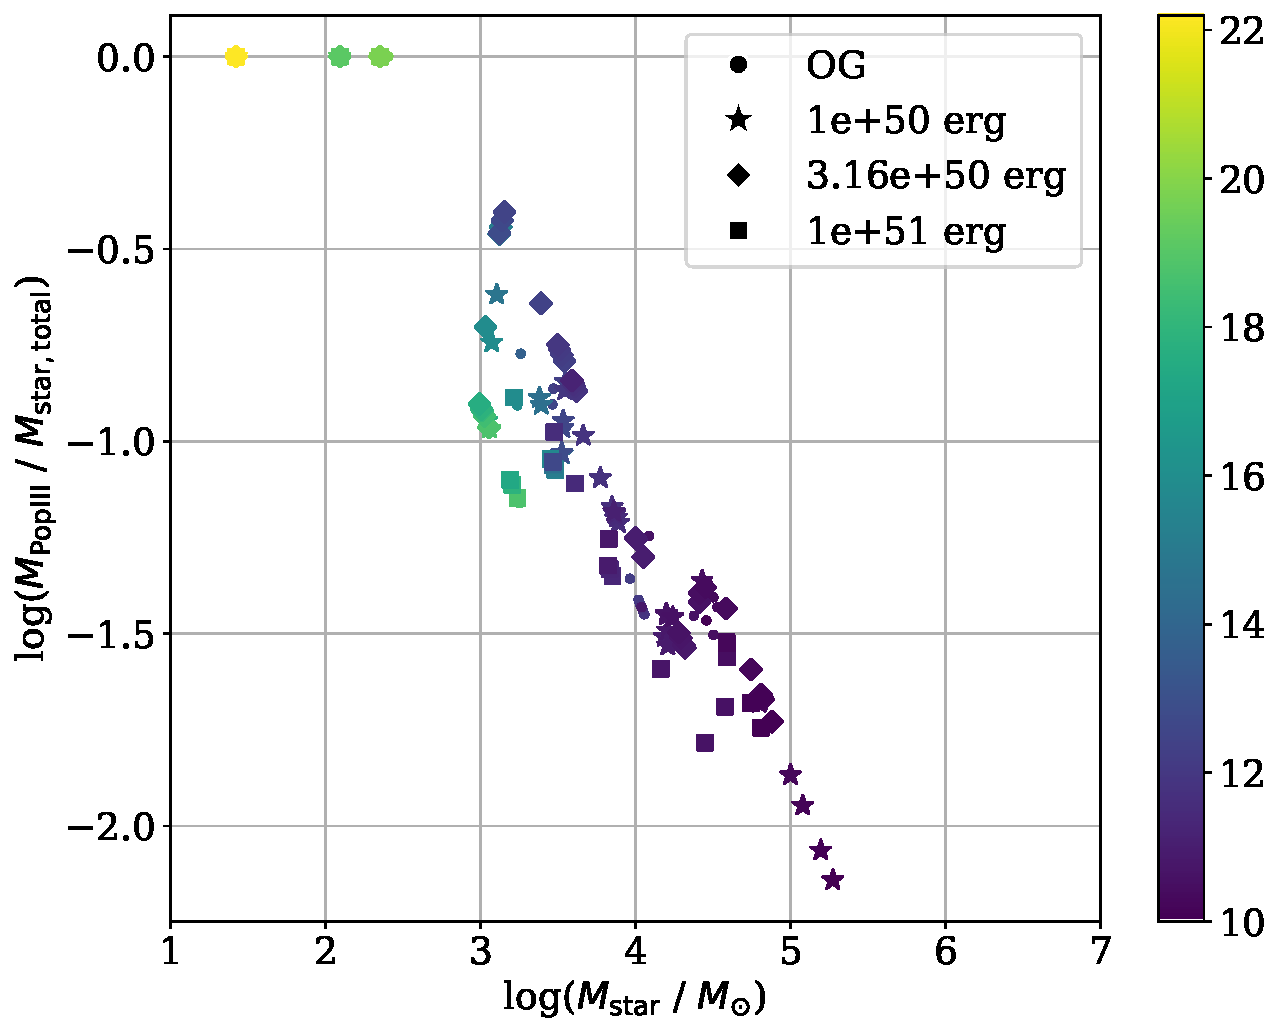
\includegraphics[width=0.4\textwidth]{plots/eng_pop3_ratio.pdf} }}%
    \qquad
    \subfloat[\centering Delay Time Variation]{{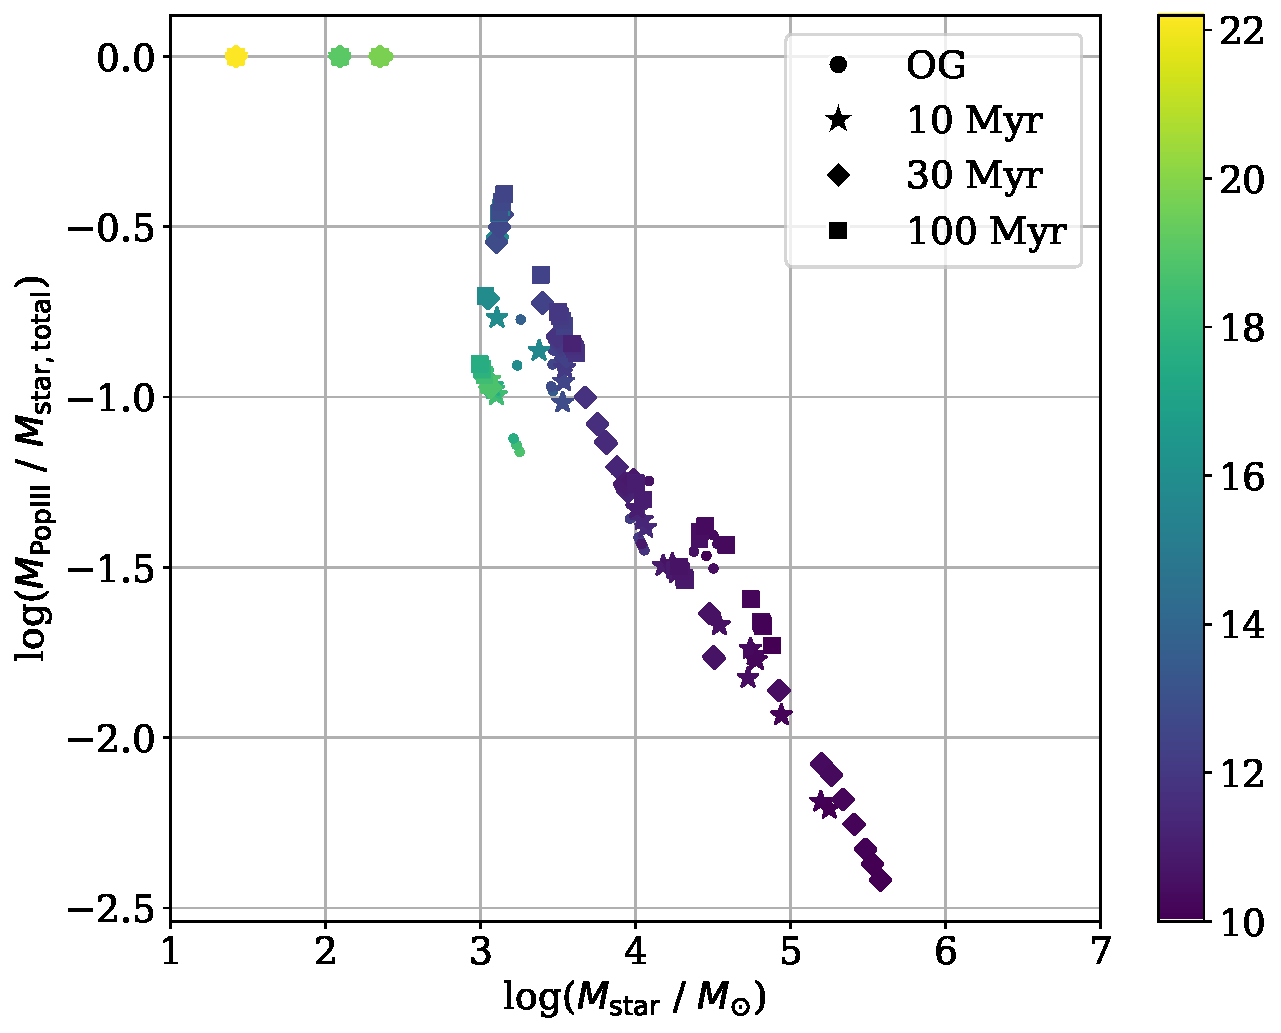
\includegraphics[width=0.4\textwidth]{plots/time_pop3_ratio.pdf} }}%
    \caption{The mass fraction of Pop III stars to total stellar mass versus the total stellar mass colored by redshift.}%
    \label{fig:ratio}%
\end{figure}

\begin{figure}[h]
    \centering
    \subfloat[\centering Energy Variation]{{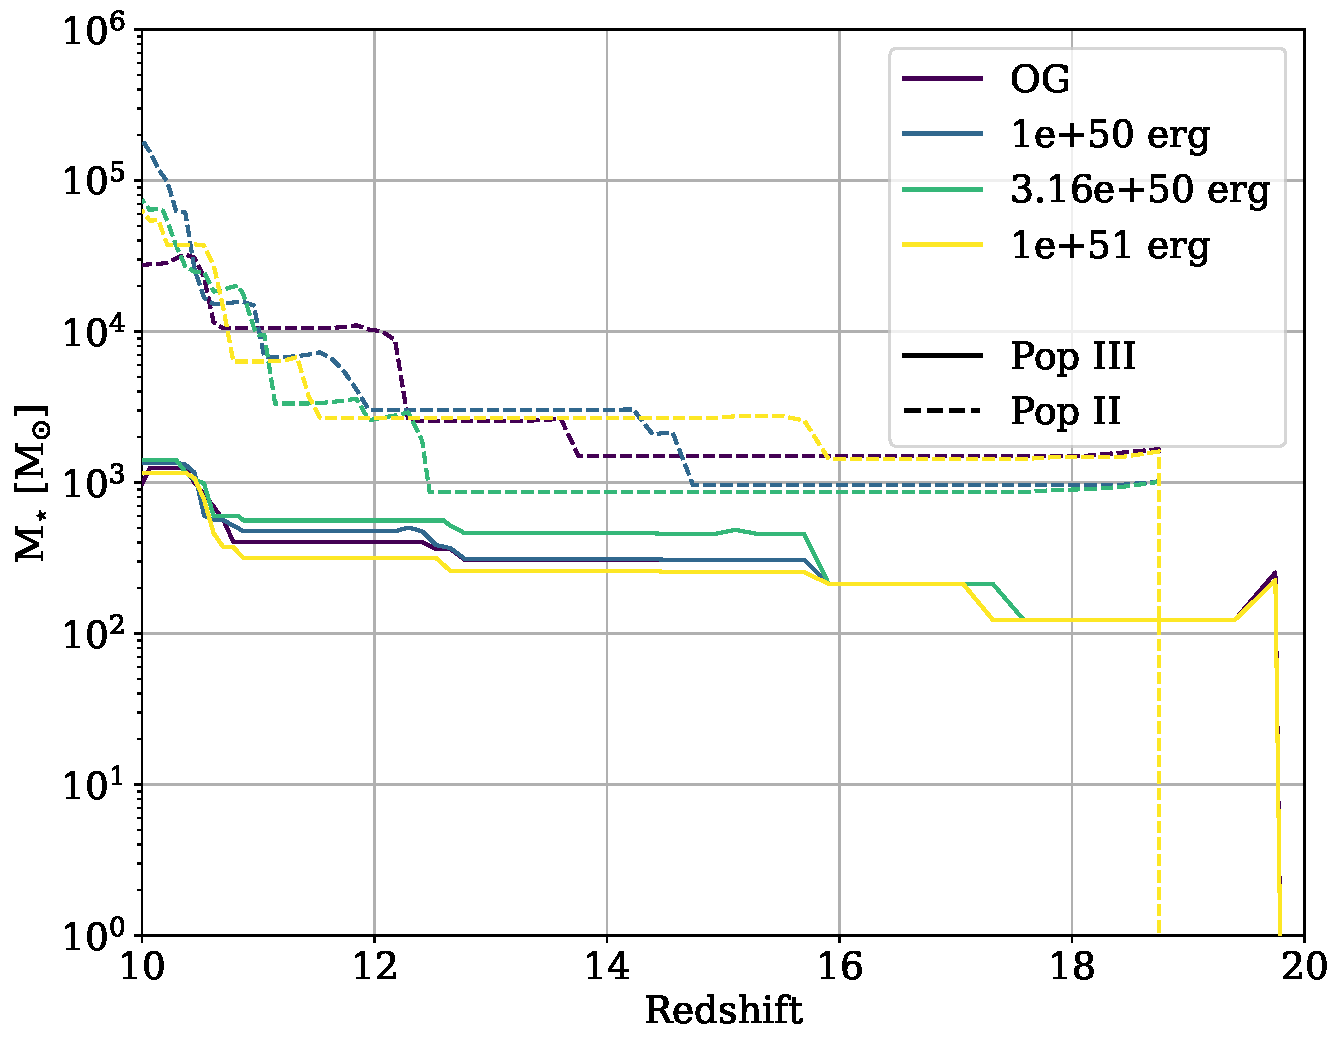
\includegraphics[width=0.4\textwidth]{plots/eng_stellar_mass.pdf} }}%
    \qquad
    \subfloat[\centering Delay Time Variation]{{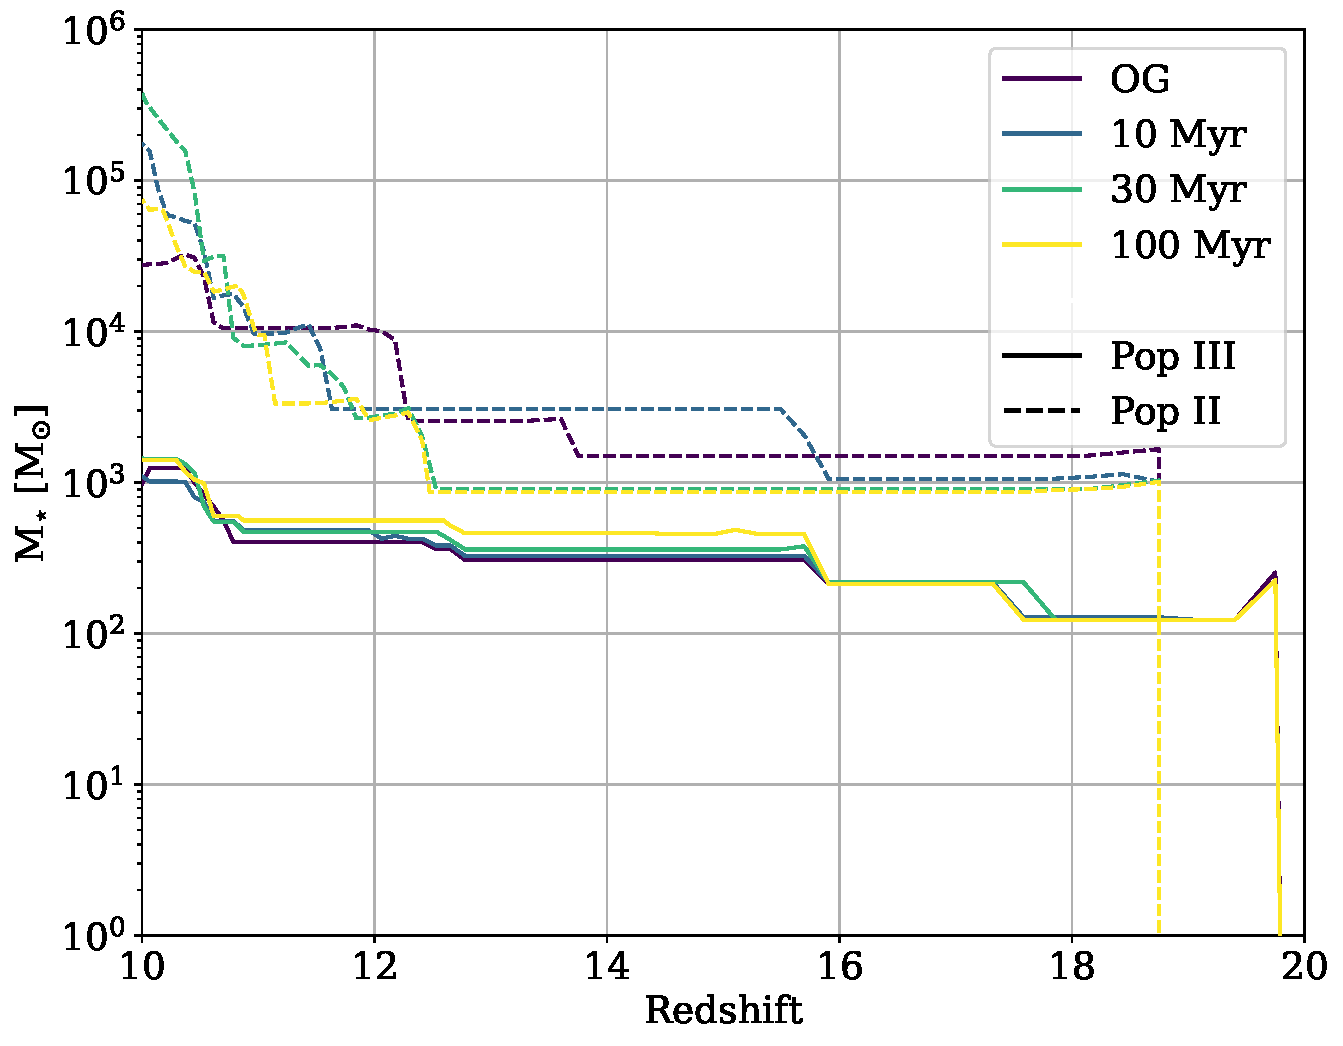
\includegraphics[width=0.4\textwidth]{plots/time_stellar_mass.pdf} }}%
    \caption{The total stellar mass of both Pop III and Pop II stars as a function of redshift. The solid lines are the total stellar masses of Pop III stars, and the dashed lines are total stellar masses of Pop II stars.}%
    \label{fig:ratio}%
\end{figure}

We again thank the referee for the insightful review that helped
improve our paper.

\bibliographystyle{plainnat}
\bibliography{drenniks}

\end{document}